\documentclass[11pt,letterpaper]{ctexart}
\usepackage{amsmath}
\usepackage{tikz}
\usepackage{epigraph}
\usepackage{lipsum}
%加入代码
\usepackage{listings}
\usepackage{xcolor}
\usepackage{color}
\usepackage{xltxtra}
\usepackage{fontspec}
\usepackage{float}
\usepackage{geometry}
\lstset{
    language=[ANSI]c,
    numbers=left,
    basicstyle=\ttfamily,%双引号可正常显示
    numberstyle={\tiny\color{lightgray}},
    keywordstyle= \color{ blue!70},
    commentstyle= \color{red!50!green!50!blue!50},
    frame=shadowbox, % 阴影效果
    rulesepcolor= \color{ red!20!green!20!blue!20} ,
    escapeinside=``, % 英文分号中可写入中文
    xleftmargin=0.5em,xrightmargin=0.5em, aboveskip=1em,
    framexleftmargin=2em,
}


\renewcommand\epigraphflush{flushright}
\renewcommand\epigraphsize{\normalsize}
\setlength\epigraphwidth{0.7\textwidth}

\definecolor{titlepagecolor}{cmyk}{1,.60,0,.40}

\DeclareFixedFont{\titlefont}{T1}{ppl}{b}{it}{0.5in}

\makeatletter
\def\printauthor{%
    {\large \@author}}
\makeatother
\author{%
    1703019班 \\
    林雪余     \\
    学号:17030199017 \\
    }

% The following code is borrowed from: https://tex.stackexchange.com/a/86310/10898

\newcommand\titlepagedecoration{%
\begin{tikzpicture}[remember picture,overlay,shorten >= -10pt]

\coordinate (aux1) at ([yshift=-15pt]current page.north east);
\coordinate (aux2) at ([yshift=-410pt]current page.north east);
\coordinate (aux3) at ([xshift=-4.5cm]current page.north east);
\coordinate (aux4) at ([yshift=-150pt]current page.north east);

\begin{scope}[titlepagecolor!40,line width=12pt,rounded corners=12pt]
\draw
  (aux1) -- coordinate (a)
  ++(225:5) --
  ++(-45:5.1) coordinate (b);
\draw[shorten <= -10pt]
  (aux3) --
  (a) --
  (aux1);
\draw[opacity=0.6,titlepagecolor,shorten <= -10pt]
  (b) --
  ++(225:2.2) --
  ++(-45:2.2);
\end{scope}
\draw[titlepagecolor,line width=8pt,rounded corners=8pt,shorten <= -10pt]
  (aux4) --
  ++(225:0.8) --
  ++(-45:0.8);
\begin{scope}[titlepagecolor!70,line width=6pt,rounded corners=8pt]
\draw[shorten <= -10pt]
  (aux2) --
  ++(225:3) coordinate[pos=0.45] (c) --
  ++(-45:3.1);
\draw
  (aux2) --
  (c) --
  ++(135:2.5) --
  ++(45:2.5) --
  ++(-45:2.5) coordinate[pos=0.3] (d);
\draw
  (d) -- +(45:1);
\end{scope}
\end{tikzpicture}%
}

\begin{document}
\begin{titlepage}

\noindent
\titlefont \indent \indent Union, Intersection\\ and Subtraction operations\\ of sets\par
\null\vfill
\vspace*{1cm}
\noindent
\hfill
\begin{minipage}{0.35\linewidth}
    \begin{flushright}
        \printauthor
    \end{flushright}
\end{minipage}
%
\begin{minipage}{0.02\linewidth}
    \rule{1pt}{125pt}
\end{minipage}

%开头装饰
\titlepagedecoration

\end{titlepage}

\tableofcontents
\newpage


    \section{需求分析}
      1.题目要求我们“编制一个能演示执行集合的并、交和差运算的程序”,即当我们输入set1 和set2后,能输出这两个集合的并集、交集和set1-set2的差。

      2.输入的要求:

\indent\indent1)集合的元素限定为小写字母['a'..'z']。但是注意输入集合中的仍可以是限定范围内的元素,只不过我们要在用户输入这些符号后剔除掉它们,只留下小写字母。

\indent\indent 2)本程序以用户用户和计算机的对话方式进行,即在计算机终端上显示“提示信息”之后,由用户在键盘上输入相应的命令和数据;相应的输出数据显示在后。

      3.输出入的要求:

      \indent\indent1)分别输出这两个集合的并集、交集和set1-set2的差。

      3.程序执行的命令包括:

      \indent\indent1)初始化单个顺序表 2)初始化输入,即两个字符集 3)合运算 4)交集运算 5)差运算

      以及两个辅助算法:

     \indent\indent 1)按升序排列集合中的元素 2)删除集合中全部的特定元素

      4.测试数据

      \indent\indent(1)题目数据

      \indent\indent(2)乱打的数据
    \section{概要设计}
    为实现上述程序功能,应以顺序表表示集合。

    1.顺序表的抽象数据类型定义为:

    ADT OrderedList{
%默认前面有个\indent,再加一个相当于重复一遍

\indent\indent   数据对象:D = \{ a$_i$ $\mid$ a$_i$ $\in$ char, i = 1, 2, \ldots,n, n$\geq$0\}

\indent\indent   数据关系:R1 = \{ <a$_{i-1}$, a$_i$> $\mid$ a$_{i-1}$,a$_i$ $\in$ D, a$_{i-1}$ < a$_i$, i = 2, \ldots,n, n$\geq$0\}

\indent\indent   基本操作:

\indent\indent\indent   InitList\underline{\hspace{0.5em}}Sq(SqList \&L)

\indent\indent\indent\indent 操作结果:初始化单个顺序表,即base指向一长串char类型的头地
\indent\indent\indent\indent 址,length == 0,listsize = LIST\underline{\hspace{0.5em}}INIT\underline{\hspace{0.5em}}SIZE。

\indent\indent\indent   InitList(SqList \&La, SqList \&Lb)

\indent\indent\indent\indent 操作结果:初始化输入 初始化set1和set2。

\indent\indent\indent   MergeList(SqList \&La,SqList \&Laa, SqList Lb,SqList \&Lc)

\indent\indent\indent\indent 初始条件:set1和set2已存在。

\indent\indent\indent\indent 操作结果:得到set1和set2的并集。

\indent\indent\indent   IntersectList(SqList La, SqList Lb, SqList Lc, SqList \&Ld)

\indent\indent\indent\indent 初始条件:set1、set2及其并集已存在。

\indent\indent\indent\indent 操作结果:得到set1和set2的交集。

\indent\indent\indent   SubtractList(SqList \&La, SqList Ld,SqList \&Lc)

\indent\indent\indent\indent 初始条件:set1已存在,并集和交集已知。

\indent\indent\indent\indent 操作结果:得到set1和set2的差集。

\indent\indent\indent   sort(SqList \&L)

\indent\indent\indent\indent 操作结果:按升序排列集合L中的元素

\indent\indent\indent   deleteCh(SqList \&La,char ch)

\indent\indent\indent\indent 操作结果:删除集合La中的特定元素

    2.结点的定义为:

\indent\indent    typedef struct\{

\indent\indent\indent	char* base;

\indent\indent\indent	int length;//集合长度 

\indent\indent\indent	int listsize;  

\indent\indent   \}SqList; 

    4.本程序包含四个模块:

    1)主程序模块

\indent\indent    int main()\{

\indent\indent\indent	SqList La,Laa,Lb,Lc,Ld;

\indent\indent\indent	//La--集合a

\indent\indent\indent	//Laa--临时集合a

\indent\indent\indent	//Lb--集合b

\indent\indent\indent	//Lc--并集

\indent\indent\indent	//ld--交集

\indent\indent\indent	InitList(La, Lb);\newline
	

\indent\indent\indent	MergeList(La,Laa,Lb,Lc);//合运算

\indent\indent\indent	IntersectList(La, Lb,Lc,Ld);//交集运算

\indent\indent\indent	SubtractList(La, Ld,Lc);//差集运算\newline

\indent\indent\indent	return 1;

\indent\indent    \}

    2)SqList模块

    3)主操作模块和辅助运算(sort和deleteCh模块)
    \section{详细设计}
  %  \newgeometry{top=0.8in,bottom=0.8in,left=1.2in,right=0.6in}
\begin{lstlisting}
#include <stdio.h>
#include <stdlib.h>
#include <string.h>

`//注意元素限定为小写字母字符['a'-'z']`
`//表内可以出现数字,但是再运算时要剔除`
`//减运算是A中减去B中有的`

#define LIST_INIT_SIZE 100

typedef struct{
 	char* base;
 	int length;`//集合长度`
 	int listsize;
}SqList;

int InitList_Sq(SqList &L);`//初始化单个顺序表`
void InitList(SqList &La, SqList &Lb);`//初始化输入`
void MergeList(SqList &La,SqList &Laa, SqList Lb,SqList &Lc);`//合运算`
void IntersectList(SqList La, SqList Lb, SqList Lc, SqList &Ld);`//交集运算`
void SubtractList(SqList &La, SqList Ld,SqList &Lc);`//差运算`

`//两个辅助算法 `
void sort(SqList &L);`//按升序排列集合中的元素`
void deleteCh(SqList &La,char ch);`//删除集合La中的特定元素`

int main(){
	SqList La,Laa,Lb,Lc,Ld;
	`//La--集合a`
	`//Laa--临时集合a`
	`//Lb--集合b`
	`//Lc--并集`
	`//ld--交集`
	InitList(La, Lb);
	
	MergeList(La,Laa,Lb,Lc);`//合运算`
	IntersectList(La, Lb,Lc,Ld);`//交集运算`
	SubtractList(La, Ld,Lc);`//差集运算`
	return 1;
}

int InitList_Sq(SqList &L){
	L.base = (char *)malloc(LIST_INIT_SIZE*sizeof(char));
	L.length = 0;
	L.listsize = LIST_INIT_SIZE;
	
	return 1;	
}

void InitList(SqList &La, SqList &Lb){
	`//初始化La`
	printf("`请输入`Set1:\n");
	char strLa[40] = {0};
	gets(strLa);
	int lenLa = strlen(strLa);
	
	int a = InitList_Sq(La);
	for(int i = 0; i < lenLa; i++){
		if('a' <= strLa[i] && strLa[i] <= 'z'){
			La.base[La.length++] = strLa[i];
		}
	}	

    `//初始化Lb`
	printf("`请输入`Set2:\n");
	char strLb[40] = {0};
	gets(strLb);
	
	InitList_Sq(Lb);
	int lenLb = strlen(strLb);
	for(int i = 0; i < lenLb; i++){
		if('a' <= strLb[i] && strLb[i] <= 'z'){
			Lb.base[Lb.length++] = strLb[i];
		}
	}	
}

void sort(SqList &L){`//排序`
	int i,pre,after,temp;
	int n = L.length;
	for( i = 0; i < n - 1; i++){
		for(pre = i, after = i + 1; after < n; after++){
			if(L.base[after] < L.base[pre]) pre = after;
		}
		
		if(pre != i){
			temp = L.base[i];
			L.base[i] = L.base[pre];
			L.base[pre] = temp;
		}
	}
}

void MergeList(SqList &La,SqList &Laa, SqList Lb,SqList &Lc){`//合运算`

	InitList_Sq(Laa);
	for(int i = 0; i < La.length; i++){`//复制`
		Laa.base[Laa.length++] = La.base[i];
	}
	
	for(int i = 0; i < Lb.length; i++){`//往Laa中插入Lb中的元素`
		if(!strchr(Laa.base,Lb.base[i])){
                    Laa.base[Laa.length++] = Lb.base[i];
           }
	}
	
	
	InitList_Sq(Lc);
	for(int i = 0; i < Laa.length; i++){`//往Lc中录入没有重复的元素`
		if(!strchr(Lc.base,Laa.base[i]))
                    Lc.base[Lc.length++] = Laa.base[i];
	}
	
	
	printf("`并集为`:\n");
	sort(Lc);
	for(int i = 0; i < Lc.length; i++){
		printf("%c",Lc.base[i]);
	}	
	printf("\n");
}

void IntersectList(SqList La, SqList Lb, SqList Lc, SqList &Ld){`//交集运算`
	InitList_Sq(Ld);
	for(int i = 0; i < Lc.length; i++){
		if((strchr(La.base,Lc.base[i]))
                && (strchr(Lb.base,Lc.base[i]))){
			Ld.base[Ld.length++] = Lc.base[i];
		}
	}
	
	if(Ld.length == 0){
		printf("`交集为:`\n`空集!`");
	}
	
	else{
		printf("`交集为`:\n");
		for(int i = 0; i < Ld.length; i++){
			printf("%c",Ld.base[i]);
		}
	}
}

void SubtractList(SqList &La, SqList Ld,SqList &Lc){
	for(int i = 0; i < Ld.length; i++){
		if(strchr(La.base,Ld.base[i])){
			deleteCh(La,Ld.base[i]);
		}
	}	
	
	InitList_Sq(Lc);
	for(int i = 0; i < La.length; i++){`//往Lc中录入没有重复的元素`
		if(!strchr(Lc.base,La.base[i]))
                    Lc.base[Lc.length++] = La.base[i];
	}
	
	printf("\n`差集为:`\n");
	sort(Lc);
	for(int i = 0; i < Lc.length; i++){
		printf("%c",Lc.base[i]);
	}
}

void deleteCh(SqList &La,char ch){`//删除a中所有的ch元素`
	for(int i = 0; i < La.length; i++){
		if(La.base[i] == ch){
			for(int j = i; j < La.length - 1; j++){`//后面的往前挪一个位置`
				La.base[j] = La.base[j+1];
			}
			La.length--;`//删去一个元素,长度要记得减一`
		}
	}
}


\end{lstlisting}
    \section{调试分析}
    1.一开始设计的用户交互界面十分不友好,没有中文提示,后来在调试下加入了用户操作提示界面,图片由用户手册中所示。

    2.一开始是用链表操作的,等到把初始化程序写好,发现集合间的运算十分麻烦,只好改用顺序表做了。这件事告诉我要事先规划好程序的框架,如何实现。不然做到半路只好再重新开始做了!
    
    3.对字符串的相关操作不熟悉,敲的时候就会想相应库了有没有这个函数呢,发现没有就很难过...
    
    4.在做合并的时候调试了许久,原因是操作中需要做到:
    
\indent\indent 1)将set1复制到Laa几何中,set1中元素保留(为之后的求差做铺垫。

\indent\indent 2)Laa中插入set2中的元素 

\indent\indent 3)往Lc(预并集中)中录入没有重复的元素 

    5.过程中有时候没有注意到字符数组的长度,会导致出bug。
    
    6.过程中求并交差集运用到了数学中集合的思想,所以每个操作比较简便。
    
    7.将一些重复的代码分装成了相应的函数,不过在运用的时候还是有些不熟悉,需要多练习。
    

    \section{用户手册}
    1.本程序的运行环境为WINDOWS系统,执行文件为集合的并、交和差运算.exe。

    2.进入演示程序后即显示文本方式的用户界面。\newpage    
\begin{figure}[ht]

\centering
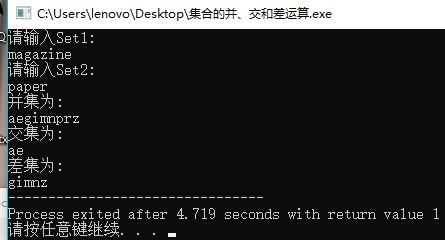
\includegraphics[scale=0.6]{a.png}
\caption{测试数据1}
\label{fig:pathdemo4}

\end{figure}

\begin{figure}[!h]

\centering
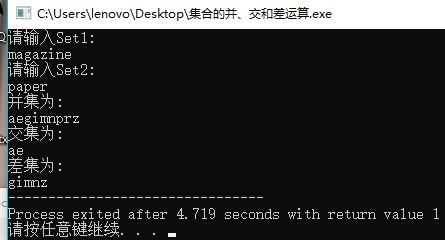
\includegraphics[scale=0.6]{a.png}
\caption{测试数据2}
\label{fig:pathdemo4}

\end{figure}

\begin{figure}[!h]

\centering
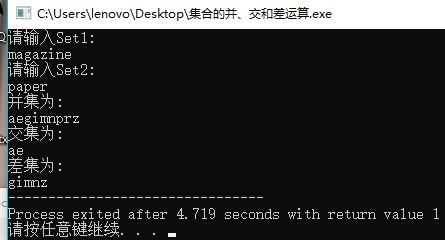
\includegraphics[scale=0.6]{a.png}
\caption{测试数据3}
\label{fig:pathdemo4}

\end{figure}


    \section{测试结果}
    测试结果如上图所示。
\end{document}
